% Template for ICASSP-2021 paper; to be used with: spconf.sty  - ICASSP/ICIP
% LaTeX style file, and IEEEbib.bst - IEEE bibliography style file.
% --------------------------------------------------------------------------
\documentclass[11pt]{article} \usepackage{spconf,amsmath,graphicx}
\usepackage{epstopdf} \usepackage{multirow} \usepackage{hyperref}
% \usepackage{fontspec}

\usepackage[utf8]{inputenc}

% Example definitions.  --------------------
\def\x{{\mathbf x}} \def\L{{\cal L}}

% Title.  ------
\title{Telugu and Tamil Speech Recognition using Transfer Learning Techniques}
%
%Single address.  ---------------
\name{Sourya Kakarla (UNI: sk5057)} \address{}



% Submit a 6-page IEEE style paper following the provided instructions.  The
% paper should include an Abstract, Introduction, State of the Art, Problem
% fromulation, your solution(s), results and discussion, and Conclusion.
\begin{document}
%\ninept
%
\maketitle
%
\begin{abstract} This project aims to develop an open-source baseline Automatic
Speech Recognition (ASR) pipeline for the Dravidian languages Tamil
and Telugu. We propose to use different speech datasets to train time-delayed
neural networks. As the total size of usable Telugu speech data (45 hours) from
these sources doesn't quite fit the requirement to achieve reasonable
performance levels, we investigate the application of transfer learning from
another Dravidian language, Tamil for which the data is relatively much more accessible. 
We present an end-to-end pipeline of taking a raw text corpus for the language model and
generating a clean dataset along with a simple tool to verify its quality.
Finally, a customized Kaldi recipe is developed by modifying the TEDLIUM one
to build the language model and train a time-delayed neural network for the acoustic modeling
using cleansed datasets and evaluate the performance of the models. In this evaluation, we also investigate the success of
using transfer learning from Tamil and English to Telugu. We aim to contribute to the low-resource open-source
ASR world and the general Speech Recognition and NLP ecosystem by publishing the
tools and techniques used in this project as a modular library after sufficient
testing and iterations.

\end{abstract}
%
\begin{keywords} automatic speech recognition, low-resource languages,
time-delayed neural networks, language model, Telugu, Tamil, open-source

\end{keywords}
%
\section{Introduction} \label{sec:intro}

\subsection{Motivation} There is a significant difference in the performance of ASR
systems for high-resource languages like English when compared to the multitude of
low-resource languages that are spoken all over the world. This is due to
various geo-political and socio-cultural aspects of the global society in the
21st century. Having said that, extensive research on natural speech and
language speech technologies is being done all over the world for a wide range
of such underserved languages. We aspire to contribute this domain, more
specifically the speech aspect by building a baseline ASR system for the
Dravidian languages, Tamil and Telugu, spoken by 81 million and 93 million
people respectively~\cite{numspeaker}.

One of the key aspects of Speech technology is it being a powerful tool to
access technology and consequently various social resources and
opportunities for the illiterate and semi-illiterate. This is especially
significant for a developing nation such as India with lower levels of literacy,
especially in rural areas. The South Indian states of Andhra Pradesh and
Telangana, for whom the predominant mother tongue is Telugu, have a literacy
rates of 72.8\% and 66.4\% respectively~\cite{literacyrate}.  This is even lower for underserved
sections of the population, such as low income sections and rural populations. 

Improving the state of the art implementations of ASR for a language like Telugu
has immense potential of improving the quality of life for many illiterate and
semi-literate. In the 21st century, the digital world has become a necessity to
lead a wellrounded life. Inspite of the integration of digital technology and
web services in many critical aspects of life in 21st century, there is a
predominant bias towards using English in the defacto implementations of systems
like Websites, Mobile Apps, IoT devices such as Google Home, Amazon Alexa etc. 

% Such a monopoly is extremely alarming and is a cause for concern as on one
% level, not having a comfortable level of English literacy deprives one of access
% to critical resources such as access to digital entities involved in education,
% public transport, welfare programs, legal and electoral processes etc. The list
% is endless due to the ubiquitous nature of technology in everyday life. 

% A practical example of the monopoly that the author has encountered is when they
% were trying to write the title of this Project Proposal Summary in their mother
% tongue, Telugu. Inspite of speaking Telugu from being an infant to their adult
% life, the author could not come up with a straight-forward translation for the
% technical term "Transfer Learning" although they are highly proficient in both
% English and Telugu that includes writing poems and songs in both languages. The
% author has tried turning to the popular translation service, Google Translate,
% to aid him. We see the result of that in Figure \ref{fig:gtranslate} 




% \begin{figure}[h]

% 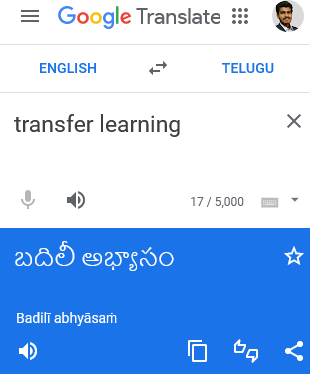
\includegraphics[width=8.5cm]{gtranslate} \caption{Attempt of translating the
% technical term "Transfer Learning" from English to Telugu using Google
% Translate} \label{fig:gtranslate}
% %
% \end{figure}

% Even if one has a moderate to high level of proficiency in English, but has a
% strong preference for using native tongue(s) in their daily life, the necessity
% to use English enforced by the existing language biases in implementation of
% technologies has strong cultural implications in the long run. It isn't
% unreasonable to say that such a bias could even lead to the extinction of
% vernacular languages throughout the world owing to monopoly of globalised
% languages such as English. This could turn out to be an irredeemable loss to
% many a culture's heritage. 

% Therefore, necessary measures need to be taken to balance the language spectrum
% in tech by creating new systems or improving existing ones that use vernacular
% languages as their defacto interface. Undoubtedly, Speech plays a crucial role
% as a medium of interaction, communication, and absorbing information. This
% project focuses on contributing to Tamil and Telugu ASR by attempting to build a
% time-delayed neural network that receives speech (Tamil/Telugu) as input and outputs a
% transcription. As Telugu has relatively less data available for training, we aim to to
% exploit transfer learning from Tamil ASR (and potentially
% English ASR too). 

To contribute towards bridging that gap, we aim to build open-source baseline ASR systems for Tamil and Telugu and investigate the effects of transfer learning on the performance of the models.
Transfer learning has proven to be quite effective in improving performance of models for related and low-resource languages as reported in multiple studies~\cite{zoph2016transfer,nguyen2017transfer,li2019cantonese}.
We take inspiration from these works and  aim to investigate using transfer learning among the Dravidian family of languages and evaluate its performance.

\section{State of the Art}
Over the last few years, there has been a surge of Indic language speech recognition studies~\cite{srivastava2018interspeech,iitmasr,Multilingual} backed by top organizations in academia and industry.
Kaldi basline WERs are reported for Tamil and Telugu by Srivastava et al.~\cite{srivastava2018interspeech} for training and test data of 40 hours and 5 hours respectively (Table~\ref{tab:kaldibaseline}).
As more data is available to us, we hope to achieve atleast a better WER than the baseline reported here.
 
\begin{table}[h]
\begin{center}
\begin{tabular}[width=5cm]{ |c|c|c|c| } 

\hline Language & GMM-HMM  & DNN & TDNN\\ \hline

Tamil & 33.55 & 25.47 & 19.45    \\  \hline

Telugu & 40.12 & 34.97 & 22.61    \\  \hline

% \multirow{2}{4em}{Malayalam} & OpenSLR~\cite{openslrtel} & 7 hours & 5.5 Hours  \\ & SMC & 1.5
% hours \\ \hline

% \multirow{1}{4em}{Kannada} & OpenSLR & 8.5 hours~\cite{openslrtel} & 8.5 hours \\ \hline


\end{tabular}

\caption{Word Error Rates of GMM-HMM, DNN and TDNN (chain) models built using the training data,
tested on the released test data~\cite{srivastava2018interspeech}}
\label{tab:kaldibaseline} \end{center} \end{table}

We can see in Fig.~\ref{fig:soa} the Word Error Rates reported in a study~\cite{javed2021towards} published in Dec, 2021. The models reported seem to be close to the top
performing ones in the field. We aspire to achieve performance as close to them as possible given our resource constraints.

\begin{figure}[h]
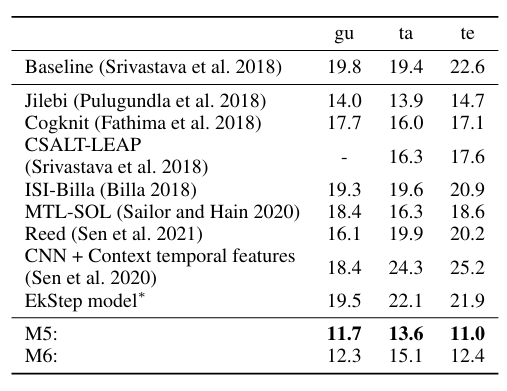
\includegraphics[width=8.5cm]{stateoftheart.png} \caption{WER comparison of the best models (M5, M6) in ~\cite{javed2021towards} with the
the top performers from the MSR 2018~\cite{srivastava2018interspeech} leaderboard as well
as other recent state of the art methods.} \label{fig:soa}
\end{figure}


 

\section{Methodology}
\subsection{Datasets}
\subsubsection{Speech}
During our investigation of publicly accessible datasets, we found that Tamil had a much larger speech
dataset available when compared to Telugu. This led us to formulate our approach
of developing a Telugu ASR model using Transfer Learning on top of layers extracted from the ASR model built for Tamil.
The speech datasets used are as follows Table \ref{tab:langdata}.


\begin{table}[h]

\begin{center}

\begin{tabular}[width=5cm]{ |c|c|c|c| } 

\hline Lang & Dataset(s) & Duration & Total\\ \hline

\multirow{3}{4em}{Telugu} & MSR Open Data~\cite{srivastava2018interspeech} & 45 h & 53.71 h  \\ & OpenSLR~\cite{openslrtel}
& 5.71 h & \\ & CMU INDIC DB~\cite{cmuindic} & 3 h & \\ \hline

\multirow{4}{4em}{Tamil} & Mozilla~\cite{cvoice} & 217.5 h & 417.5 h \\ & IITM~\cite{iitmasr} & 118 h &  \\ & MSR Open Data~\cite{srivastava2018interspeech}
& 45 h & \\ & OpenSLR~\cite{openslrtel} & 7.5 h & \\ \hline

% \multirow{2}{4em}{Malayalam} & OpenSLR~\cite{openslrtel} & 7 hours & 5.5 Hours  \\ & SMC & 1.5
% hours \\ \hline

% \multirow{1}{4em}{Kannada} & OpenSLR & 8.5 hours~\cite{openslrtel} & 8.5 hours \\ \hline
\end{tabular}
\caption{Publicly available speech datasets of Tamil and Telugu Languages}
\label{tab:langdata} \end{center} \end{table}

\subsubsection{Language Modeling} 
Though we had the option to use pre-built open-source language models, we took a raw corpus of Tamil and Telugu by IndicCorp~\cite{kakwani2020indicnlpsuite}
which was built by scraping thousands of web sources - primarily news, magazines and books, over a duration of several months. Their statistics are presented in Table ~\ref{tab:langmodel}.

\begin{table}[h]
\begin{center}
\begin{tabular}[width=5cm]{ |c|c|c|c| } 
\hline Lang & \# Articles & Sentences & Tokens\\ \hline
ta~\cite{tamilkakwani2020indicnlpsuite} & 4.41M & 31.5M & 582M\\ \hline
te~\cite{telugukakwani2020indicnlpsuite} & 3.98M & 47.9M & 674M\\ \hline


% \multirow{2}{4em}{Malayalam} & OpenSLR~\cite{openslrtel} & 7 hours & 5.5 Hours  \\ & SMC & 1.5
% hours \\ \hline

% \multirow{1}{4em}{Kannada} & OpenSLR & 8.5 hours~\cite{openslrtel} & 8.5 hours \\ \hline


\end{tabular}

\caption{Tamil and Telugu text corpora used for language modeling}
\label{tab:langmodel} \end{center} \end{table}

\subsection{Github Repository}
With the aim of contributing to the open-source community eventually, we created 3 Github repositories which are as follows:
\begin{itemize}
	\item \textbf{speech\_rec}~\cite{speech_rec}: This is the main repository for the project. The other two repositories are submodules of this repository.
	Most of the data preprocessing and handling modules are implemented in this repository.
	\item \textbf{kaldi\_tamtel}~\cite{kalditamtel}: In this repository, the Kaldi recipe for Tamil and Telugu customized from the Tedlium recipe is hosted.
	 Logs~\cite{logs} are maintained for most of the steps in entire pipeline of the recipe. This is a repository for the project. The other two repositories are submodules of this repository.
	\item \textbf{kaldi\_tamtel\_db}~\cite{kaldidb}: In this repository, the Kaldi data files which are input to Kaldi and are generated by various stages of the pipeline are hosted to keep track of changes.
	Although files which are too big for Github are not hosted as of now. 
\end{itemize}

We have first started working on the Tamil part of the project. At the time of the submission, we haven't yet started working on the Telugu part explicitly.
Therefore, in the following sections, most of the work will be focused on Tamil. Yet, it is easy to see that it can be extended to Telugu as well with minimal effort
and complexity.

\subsection{Preprocessing for language modeling}
As the transcripts and corpora used for language modeling had a lot of undesirable entities like english words, punctuation, special characters etc.,
we devised a preprocessing pipeline~\cite{cleancorpus} to remove these entities and to produce clean datasets. The salient features of the preprocessing steps are:
\begin{itemize}
	\item \textbf{Repleace numbers with words}: Numbers written as numerals are converted to words using the \texttt{replace\_num.sh}~\cite{num2wordsscript} script.
	This script uses the \texttt{indic-num2words}~\cite{num2wordsscript} module to get the words(s) for a given number in the given Indian language.
	% \begin{itemize}
		% \item Example - Tamil: 23 --- இருபத்து மூன்று
	% 	% \item Example - Telugu: 23 --- ఒకటిఇరువై మూడు
	% 	\item Example - Tamil: 23 ---  
	% 	\item Example - Telugu: 23 --- {\tel నమో పకవతే నారాయణాయ!}
	% \end{itemize}
	\item \textbf{Remove URLs}: As the text contained urls, they had to be removed.
	\item \textbf{Remove parentheses}: Various kinds of parentheses and their contents are removed from the text.
	\item \textbf{Remove punctuation and special characters}: Punctuation and special characters except for periods are removed.
	\item \textbf{Remove parentheses}: Various kinds of parentheses and their contents are removed from the text.
	This script uses the \texttt{indic-num2words} module to get the words(s) for a given number in the given Indian language.
	\item \textbf{Remove non-language and whitespace character}: This step is kind of a fail safe. All characters except for the unicode range of the language and whitespace are replaced by a space.
	This step is kind of a fail safe as it is guaranteed to catch anything that's not caught in the above steps. It is to be ensured that the data is cleaned and adapted
	as much as possible before this step. 
	\item \textbf{Convert periods into newlines}: As PocoLM uses newlines as the delimiter, we need to convert the periods into newlines.
	\item \textbf{Delete empty lines}: There is a possibility that some lines are empty after the above steps. These lines are deleted.
	\item \textbf{Fix whitespace}: Make sure there are no leading or trailing whitespace in each line. Make sure that there are no multiple whitespaces in each line.
	\item \textbf{Validate end result}: Each line of the corpus is checked whether it contains only tamil words that are separated by a single space without any leading or trailing whitespace.
	It is also verified that there are no empty lines in the processed corpus. Instead of verifying on the whole corpus, a random sample of 25k lines~\cite{randnsample} is extracted out of the processed corpus and the
	validation is run using the \texttt{validate\_text\_file.sh} script~\cite{validatecorpus}.
\end{itemize}


\subsection{Preprocessing Speech Dataset}
The transcript texts of the audio are preprocessed similar to the steps outlined above for the most part. Therefore, skipping the details for brevity.
As we have 4 different datasets, it's vital to have the audio files in standard format. The audio files are handled as follows:
\begin{itemize}
	\item Convert all files to \texttt{wav} format using soxi 
	\begin{itemize}
		\item Sample Rate : 16000
		\item Precision : 16-bit
		\item Sample Encoding: 16-bit Signed Integer PCM
	\end{itemize}
	\item Prepare data (input files to Kaldi) for each of the datasets in the required formats with the standard \texttt{dev, test, train} partition.
	This is done using the \texttt{create\_data\_files.py} module~\cite{createfiles}.
	\item Merge the data files for each of the datasets into a single unified dataset (with the partitions). Implemented in \texttt{merge\_datasets.sh} script~\cite{mergedb}.
	\item \textbf{Create lexicon:} Significant effort was spent on using a unified parser~\cite{baby2016unified} which would spell out phonemes in a uniform format for multiple Indian languages.  phonemesMerge the data files for each of the datasets into a single unified dataset (with the partitions). 
	We weren't able to get it working in time and we move on to simply splitting a word into its constituent unicode characters and treated that list as the pronunciation oh phonemes.
	This is implemented in \texttt{create\_lexicon.py} module~\cite{createlexicon} and a snippet is shown in Fig. ~\ref{fig:lexicon}.
	\begin{figure}[h]

	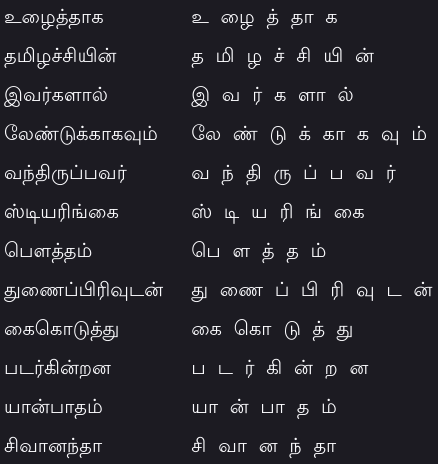
\includegraphics[width=8.5cm]{lexicon} \caption{Snippet of lexicon created by spiltting characters} \label{fig:lexicon}

	\end{figure}



\end{itemize}

\subsection{Customizing Tedlium Recipe}
We copy the Tedlium \texttt{s5\_r3} folder into the \texttt{egs} folder of Kaldi and start making changes to build the recipe~\cite{kalditamtel} for our project.
The changes are as follows:
\begin{itemize}
	\item \textbf{Adapting data path and initial stages}: The merged Kaldi input data from the above is placed in the \texttt{db} folder and relevant changes are made to the data download
	\item \textbf{Run utils/fix\_data\_dir.sh}: There seemed to have been a sorting issue in the data directory. This utility script is run to fix the issue.
	\item \textbf{Language model script}: \texttt{ted\_train\_lm.sh} is modified into \texttt{tamil\_train\_lm.sh} with it being pointed to the relevant data files to pick the data extracted after preprocessing.
	\item \textbf{Fix PocoLM script(s) encoding bug}: A few scripts like \texttt{prepare\_int\_data} were failing due to an encoding issue~\cite{encodingbug} in calling the method \texttt{subprocess.check\_output}. This is fixed by adding the parameter \texttt{encoding='utf-8'} to the method in the PocoLM scripts.
\end{itemize}

\subsection{Running the stages of the recipe for Tamil}
\subsection{Language Model Training}
We were successful in building the language model (Stages 4 and 5) using the training text obtained after the earlier mentioned preprocessing.
The following are the perplexity values for the language model:
\begin{table}[h]
\begin{center}
\begin{tabular}[width=5cm]{ |c|c|c|c| } 
\hline Model & Log-Prob per Word & Perplexity\\ \hline
lm\_4\_prune\_big~\cite{prunebig} &  -7.93  & 2785.2\\ \hline
lm\_4\_prune\_small~\cite{prunesmall} &   8.40  & 4472.5\\ \hline


% \multirow{2}{4em}{Malayalam} & OpenSLR~\cite{openslrtel} & 7 hours & 5.5 Hours  \\ & SMC & 1.5
% hours \\ \hline

% \multirow{1}{4em}{Kannada} & OpenSLR & 8.5 hours~\cite{openslrtel} & 8.5 hours \\ \hline


\end{tabular}

\caption{Log-Probability per Word and Perplexity calculated for the language models over 109506 words on \texttt{real\_dev\_set.txt}}
\label{tab:resultslangmodel} \end{center} \end{table}
\begin{itemize}
	\item 
\end{itemize}

\subsection{Acousting Model Training}
We were able to run all stages upto the stage 12 (of Tedlium recipe) successfully (eventually).  During this process, we  were halted by a few errors in the earlier stages
which we were able to fix with some debugging and some minor changes. At the time of writing this report, we are debugging an issue with \texttt{sort} in Stage 13.

\section{Results}
Due to the above mentioned situation, we aren't able to report any comprehensive results apart from building the language model from scratch using a raw corpus.
We will keep working on finishing the outlined goals and report more results in a later communication.

\section{Conclusion}
As mentioned above, we don't have any conclusions with any closure yet  apart from an understanding of the Kaldi pipeline and the Tedlium recipe.
In addition to that, we have designed and implemented necessary preprocessing techniques used on corpora to build language models.

\section{Pending/Future Work}
\begin{itemize}
	\item Finish acoustic modeling training and evaluation for Tamil.
	\item Run the same recipe adapted to Telugu
	\item Investigate using layers from Tamil/English neural networks for Telugu
	\item If possible, extend to other Dravidian languages like Kannada, Malayalam, etc.
\end{itemize}

% -------------------------------------------------------------------------
\bibliographystyle{IEEEbib} \bibliography{strings,refs}

\end{document}
